\nsection{Data structures}

% \subsection{Disjoint set}
% \addfile{../Codes/DataStructures/DSU.cpp}

\subsection{Disjoint set with rollback}
\addfile{../Codes/DataStructures/DSURollback.cpp}

\subsection{Sparse table}
\addfile{../Codes/DataStructures/SparseTable.cpp}

% \subsection{RMQ}
% \addfile{../Codes/DataStructures/RMQ.cpp}

\subsection{Min-Max queue}
\addfile{../Codes/DataStructures/MinMaxQueue.cpp}

\subsection{Squirtle decomposition}
\vspace{-18pt}
\begin{minipage}{70mm}
  The perfect block size is $squirtle$ of N
\end{minipage}
\begin{minipage}{15mm}
  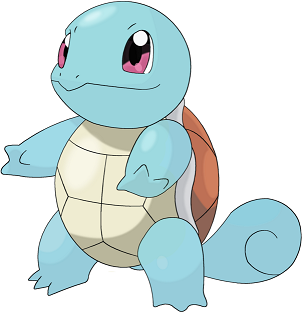
\includegraphics[width=\linewidth]{squirtle.png} 
\end{minipage}
\addfile[]{../Codes/DataStructures/SqrtDecomposition.cpp}
\vspace{-18pt}

\subsection{In-Out trick}
\addfile{../Codes/DataStructures/InOutTrick.cpp}

\subsection{Parallel binary search}
\addfile{../Codes/DataStructures/ParallelBinarySearch.cpp}

\subsection{Mo's algorithm}
\addfile{../Codes/DataStructures/Mos.cpp}
To make it faster, change the order to $hilbert(l, r)$ \\
\addfile{../Codes/DataStructures/HilbertOrder.cpp}

\subsection*{Mo's algorithm with updates in \complexity{n^{\frac{5}{3}}} }
  
\setlist{nolistsep}
\begin{itemize}[noitemsep]
  \item Choose a $block$ of size $n^{\frac{2}{3}}$
  \item Do a normal Mo's algorithm, in the $Query$ definition add an extra variable for the $updatesSoFar$ 
  \item Sort the queries by the order $(l /block$, $r / block$, $updatesSoFar)$
  \item If the update lies inside the current query, update the data structure properly \\
  \begin{code}
   struct Update {
     int pos, prv, nxt;
   };
  
   void undo(Update &u) {
     if (l <= u.pos && u.pos <= r) {
       rem(u.pos);
       a[u.pos] = u.prv;
       add(u.pos);
     } else {
       a[u.pos] = u.prv;
     }
   }
  \end{code}
    
  \item Solve the problem :D \\
  \begin{code}
   l = queries[0].l, r = l - 1, upd = sz(updates) - 1;
   for (Query &q : queries) {
     while (upd < q.upd)
       dodo(updates[++upd]);
     while (upd > q.upd)
       undo(updates[upd--]);
     // write down the normal Mo's algorithm
   }
  \end{code}
\end{itemize}

\subsection{Ordered tree}
\addfile{../Codes/DataStructures/OrderedTree.cpp}

\subsection{Unordered tree}
\addfile[4]{../Codes/DataStructures/UnorderedTree.cpp}

\subsection{D-dimensional Fenwick tree}
\addfile[1-28]{../Codes/DataStructures/FenwickND.cpp}

% \subsection{Segment tree}
% \addfile{../Codes/DataStructures/Segtree.cpp}

% \subsection{Lazy segment tree}
% \addfile{../Codes/DataStructures/LazySegtree.cpp}

\subsection{Dynamic segment tree}
\addfile{../Codes/DataStructures/DynamicSegtree.cpp}

\subsection{Persistent segment tree}
\addfile{../Codes/DataStructures/PersistentSegtree.cpp}

\subsection{Wavelet tree}
\addfile{../Codes/DataStructures/Wavelet.cpp}

\subsection{Li Chao tree}
\addfile{../Codes/DataStructures/LiChao.cpp}

\subsection{Treap}
\addfile{../Codes/DataStructures/Treap.cpp}